\documentclass[notes,11pt, aspectratio=169]{beamer}

\usepackage{pgfpages}
\setbeameroption{hide notes} % Only slide

\usepackage{array}
\usepackage{tikz}
\usepackage{verbatim}
\setbeamertemplate{note page}{\pagecolor{gray!5}\insertnote}
\usetikzlibrary{positioning}
\usetikzlibrary{snakes}
\usetikzlibrary{calc}
\usetikzlibrary{arrows}
\usetikzlibrary{decorations.markings}
\usetikzlibrary{shapes.misc}
\usetikzlibrary{matrix,shapes,arrows,fit,tikzmark}
\usepackage{amsmath}
\usepackage{mathpazo}
\usepackage{hyperref}
\usepackage{lipsum}
\usepackage{multimedia}
\usepackage{graphicx}
\usepackage{multirow}
\usepackage{dcolumn}
\usepackage{bbm}
\newcolumntype{d}[0]{D{.}{.}{5}}

\usepackage{changepage}
\usepackage{appendixnumberbeamer}

\usepackage[space]{grffile}
\usepackage{booktabs}

% Colors
\definecolor{blue}{RGB}{0,114,178}
\definecolor{red}{RGB}{213,94,0}
\definecolor{yellow}{RGB}{240,228,66}
\definecolor{green}{RGB}{0,158,115}
\definecolor{solutionbg}{RGB}{240,248,240}
\definecolor{solutionframe}{RGB}{0,158,115}

% Solution box environment for worked answers
\usepackage{tcolorbox}
\newtcolorbox{solutionbox}[1][]{
  enhanced,
  colback=solutionbg,
  colframe=solutionframe,
  boxrule=0pt,
  leftrule=3pt,
  arc=0pt,
  left=8pt,
  right=8pt,
  top=6pt,
  bottom=6pt,
  fonttitle=\bfseries,
  title={#1},
  attach boxed title to top left={yshift=-2mm, xshift=5mm},
  boxed title style={colback=solutionframe, colframe=solutionframe, size=small, arc=2pt}
}

\hypersetup{
  colorlinks=false,
  linkbordercolor = {white},
  linkcolor = {blue}
}

\definecolor{MyBackground}{RGB}{255,253,218}

\newenvironment{transitionframe}{
  \setbeamercolor{background canvas}{bg=white}
  \begin{frame}}{
    \end{frame}
}

\setbeamercolor{frametitle}{fg=blue}
\setbeamercolor{title}{fg=black}
\setbeamertemplate{footline}[frame number]
\setbeamertemplate{navigation symbols}{}
\setbeamertemplate{itemize items}{-}
\setbeamercolor{itemize item}{fg=blue}
\setbeamercolor{itemize subitem}{fg=blue}
\setbeamercolor{enumerate item}{fg=blue}
\setbeamercolor{enumerate subitem}{fg=blue}
\setbeamercolor{button}{bg=MyBackground,fg=blue,}

\setbeamercolor{section in toc}{fg=blue}
\setbeamercolor{subsection in toc}{fg=red}
\setbeamersize{text margin left=1em,text margin right=1em}

\newenvironment{wideitemize}{\itemize\addtolength{\itemsep}{10pt}}{\enditemize}
\newenvironment{wideenumerate}{\enumerate\addtolength{\itemsep}{10pt}}{\endenumerate}

\title[]{\textcolor{blue}{ECN 594: Consumer Surplus, IIA, and Price Discrimination}}
\author[PGP]{}
\institute[FRBNY]{\small{\begin{tabular}{c c c}
Nicholas Vreugdenhil \\
\end{tabular}}}
\date{\today}

\begin{document}

% Title Slide
\begin{frame}
\maketitle
  \centering
\end{frame}

\begin{frame}{Plan for today}
  \begin{wideenumerate}
    \item \textbf{Consumer surplus: the log-sum formula}
    \item The IIA problem: Red Bus / Blue Bus
    \item From demand to supply
    \item Types of price discrimination
    \item Selection by indicators
    \item Worked example: optimal pricing across markets
  \end{wideenumerate}
\end{frame}

%%%%%%%%%%%%%%%%%%%%%%%%%%%%%%%%%%%%%%%%%%%%%%%%%%%%%%%%%%%%%
% CONSUMER SURPLUS AND IIA
%%%%%%%%%%%%%%%%%%%%%%%%%%%%%%%%%%%%%%%%%%%%%%%%%%%%%%%%%%%%%

\begin{frame}{Why do we care about consumer surplus?}
	\begin{wideitemize}
		\item Policy analysis requires measuring welfare
		\item Questions we want to answer:
		\begin{wideitemize}
			\vspace{5pt}
			\item How much do consumers gain from a new product?
			\item How much do consumers lose from a merger?
			\item What is the welfare cost of a price increase?
		\end{wideitemize}
		\item Need a way to compute consumer surplus from our demand model
	\end{wideitemize}
\end{frame}

\begin{frame}{Consumer surplus in logit: the log-sum formula}
	\begin{wideitemize}
		\item For consumer $i$, expected utility from choosing among $J$ products:
		\begin{align*}
			E[\max_j u_{ij}] = \ln\left[\sum_{j=0}^J \exp(\delta_j + \mu_{ij})\right] + \text{constant}
		\end{align*}
		\item This is the ``log-sum'' or ``inclusive value''
		\item Consumer surplus (in dollars):
		\begin{align*}
			CS_i = \frac{1}{\alpha} \ln\left[\sum_{j=0}^J \exp(\delta_j + \mu_{ij})\right]
		\end{align*}
		\item Divide by $\alpha$ (price coefficient) to convert to dollars
	\end{wideitemize}
\end{frame}

\begin{frame}{Intuition for the log-sum}
	\begin{wideitemize}
		\item Think of choosing the best option as a lottery
		\item Each product gives you a random utility draw
		\item \textbf{Expected value of the BEST draw} is the log-sum
		\item Key insights:
		\begin{wideitemize}
			\vspace{5pt}
			\item More options $\rightarrow$ higher CS (more lottery tickets)
			\item Better options $\rightarrow$ higher CS (higher $\delta_j$)
			\item Higher price sensitivity $\rightarrow$ divide by larger $\alpha$
		\end{wideitemize}
	\end{wideitemize}
\end{frame}

\begin{frame}{Worked example: CS change from price increase}
	\begin{wideitemize}
		\item \textbf{Question:}
		\item Two products with $\delta_1 = 2$ and $\delta_2 = 1$. Outside option $\delta_0 = 0$.
		\item Price coefficient $\alpha = 0.8$.
		\item If product 1's price increases by \$2 (so $\delta_1$ falls to 0.4), what is the CS loss?
	\end{wideitemize}
	\vspace{15pt}
	\centering
	\textit{Take 3 minutes to solve this.}
\end{frame}

\begin{frame}{Worked example: CS change from price increase (solution)}
	\begin{solutionbox}[Solution]
		\begin{itemize}
			\item Note: $\Delta \delta_1 = -\alpha \times \Delta p = -0.8 \times 2 = -1.6$, so new $\delta_1 = 2 - 1.6 = 0.4$
			\item \textbf{Before:}
			\begin{align*}
				CS^{\text{before}} = \frac{1}{0.8} \ln(e^0 + e^2 + e^1) = 1.25 \ln(1 + 7.39 + 2.72) = 1.25 \times 2.41 = 3.01
			\end{align*}
			\item \textbf{After:}
			\begin{align*}
				CS^{\text{after}} = \frac{1}{0.8} \ln(e^0 + e^{0.4} + e^1) = 1.25 \ln(1 + 1.49 + 2.72) = 1.25 \times 1.65 = 2.06
			\end{align*}
			\item \textbf{Loss:} $3.01 - 2.06 = \$0.95$ per consumer
		\end{itemize}
	\end{solutionbox}
\end{frame}

\begin{frame}{Worked example: CS change from removing a product}
	\begin{wideitemize}
		\item \textbf{Question:} Market has 2 products with $\delta_1 = 1$, $\delta_2 = 0.5$. Outside option has $\delta_0 = 0$. Suppose $\alpha = 0.5$.
		\item What is the consumer surplus loss if product 1 is removed?
	\end{wideitemize}
	\vspace{15pt}
	\centering
	\textit{Take 3 minutes to solve this.}
\end{frame}

\begin{frame}{Worked example: CS change (solution)}
	\begin{solutionbox}[Solution]
		\begin{itemize}
			\item \textbf{Before removal:}
			\begin{align*}
				CS^{\text{before}} = \frac{1}{0.5} \ln(e^0 + e^1 + e^{0.5}) = 2 \ln(1 + 2.72 + 1.65) = 2 \ln(5.37) = 3.36
			\end{align*}
			\item \textbf{After removal:}
			\begin{align*}
				CS^{\text{after}} = \frac{1}{0.5} \ln(e^0 + e^{0.5}) = 2 \ln(1 + 1.65) = 2 \ln(2.65) = 1.95
			\end{align*}
			\item \textbf{Loss:} $3.36 - 1.95 = 1.41$ dollars per consumer
			\item This is on HW1!
		\end{itemize}
	\end{solutionbox}
\end{frame}

\begin{frame}{Plan for today}
  \begin{wideenumerate}
    \item Consumer surplus: the log-sum formula
    \item \textbf{The IIA problem: Red Bus / Blue Bus}
    \item From demand to supply
    \item Types of price discrimination
    \item Selection by indicators
    \item Worked example: optimal pricing across markets
  \end{wideenumerate}
\end{frame}

\begin{frame}{The IIA problem: Red Bus / Blue Bus}
	\begin{wideitemize}
		\item \textbf{Setup:} Consumers choose how to commute
		\item Choices: Car, Red Bus
		\item Suppose: half choose Car, half choose Red Bus
		\item So: $\delta_{\text{car}} = \delta_{\text{red bus}} = 0$
	\end{wideitemize}
\end{frame}

\begin{frame}{Red Bus / Blue Bus: introducing a new option}
	\begin{wideitemize}
		\item Now introduce a \textbf{Blue Bus}
		\item But consumers are color-blind!
		\item Blue Bus is identical to Red Bus in every way
		\item \textbf{Reality:} Welfare should NOT change
		\begin{wideitemize}
			\vspace{5pt}
			\item It's the same bus, just different color
			\item No real new option
		\end{wideitemize}
	\end{wideitemize}
\end{frame}

\begin{frame}{What does logit predict?}
	\begin{wideitemize}
		\item \textbf{Before Blue Bus:}
		\begin{align*}
			\text{Inclusive value} = \ln(e^0 + e^0) = \ln(2)
		\end{align*}
		\item \textbf{After Blue Bus:} $\delta_{\text{blue bus}} = \delta_{\text{red bus}} = 0$
		\begin{align*}
			\text{Inclusive value} = \ln(e^0 + e^0 + e^0) = \ln(3)
		\end{align*}
		\item Logit says welfare \textbf{increased}!
		\item But nothing real changed...
	\end{wideitemize}
\end{frame}

\begin{frame}{The IIA problem: what went wrong?}
	\begin{wideitemize}
		\item Logit gives an extra ``lottery ticket'' for each product
		\item It doesn't know that buses are close substitutes
		\item \textbf{IIA:} The ratio $s_j/s_k$ doesn't depend on other options
		\begin{align*}
			\frac{s_{\text{car}}}{s_{\text{red bus}}} = \frac{e^0}{e^0} = 1 \quad \text{(before and after!)}
		\end{align*}
		\item Adding Blue Bus steals equally from Car and Red Bus
		\item But Car and Red Bus are NOT equally similar to Blue Bus
	\end{wideitemize}
\end{frame}

\begin{frame}{Red Bus / Blue Bus: The math}
	\begin{wideitemize}
		\item \textbf{Before} (Car, Red Bus): $s_{\text{car}} = s_{\text{red}} = 0.5$
		\item \textbf{After} (Car, Red Bus, Blue Bus), logit predicts:
		\begin{align*}
			s_{\text{car}} = \frac{e^0}{e^0 + e^0 + e^0} = \frac{1}{3}
		\end{align*}
		\item Car's share dropped from 0.5 to 0.33!
		\item \textbf{Reality:} Car share should stay at 0.5
		\begin{wideitemize}
			\vspace{5pt}
			\item Car commuters don't care about bus color
			\item Blue Bus should only steal from Red Bus
		\end{wideitemize}
	\end{wideitemize}
\end{frame}

\begin{frame}{Red Bus / Blue Bus: Visual}
	\begin{center}
	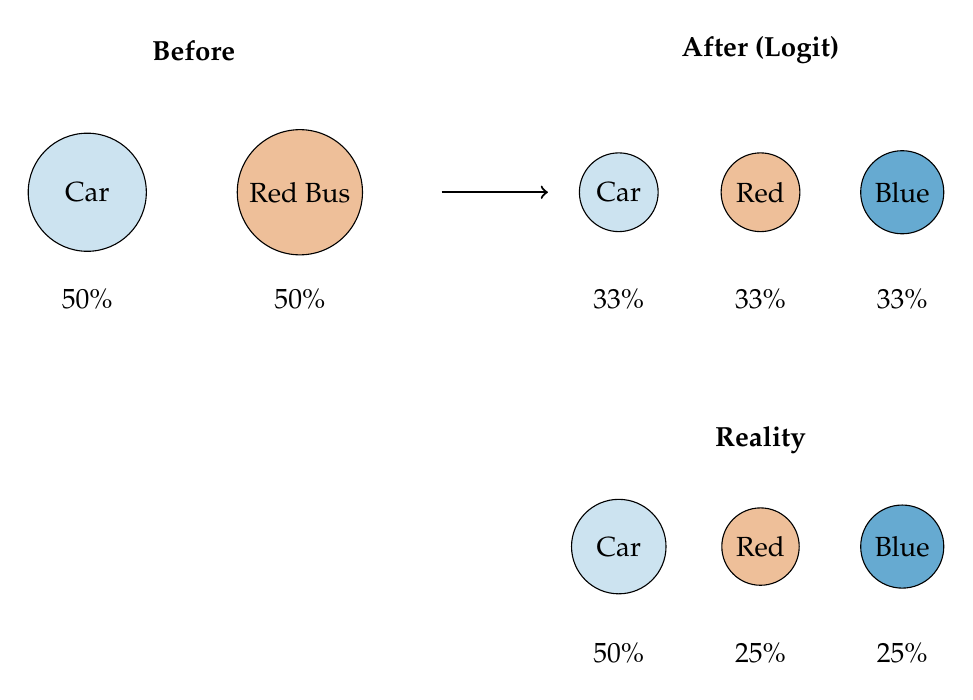
\begin{tikzpicture}[scale=0.9]
		% Before panel
		\node at (0, 3.5) {\textbf{Before}};
		\node[draw, circle, minimum size=1.5cm, fill=blue!20] (car1) at (-1.5, 1.5) {Car};
		\node[draw, circle, minimum size=1.5cm, fill=red!40] (rbus1) at (1.5, 1.5) {Red Bus};
		\node at (-1.5, 0) {50\%};
		\node at (1.5, 0) {50\%};

		% Arrow
		\draw[->, thick] (3.5, 1.5) -- (5, 1.5);

		% After panel - Logit prediction
		\node at (8, 3.5) {\textbf{After (Logit)}};
		\node[draw, circle, minimum size=1cm, fill=blue!20] (car2) at (6, 1.5) {Car};
		\node[draw, circle, minimum size=1cm, fill=red!40] (rbus2) at (8, 1.5) {Red};
		\node[draw, circle, minimum size=1cm, fill=blue!60] (bbus2) at (10, 1.5) {Blue};
		\node at (6, 0) {33\%};
		\node at (8, 0) {33\%};
		\node at (10, 0) {33\%};

		% Reality panel
		\node at (8, -2) {\textbf{Reality}};
		\node[draw, circle, minimum size=1.2cm, fill=blue!20] (car3) at (6, -3.5) {Car};
		\node[draw, circle, minimum size=0.8cm, fill=red!40] (rbus3) at (8, -3.5) {Red};
		\node[draw, circle, minimum size=0.8cm, fill=blue!60] (bbus3) at (10, -3.5) {Blue};
		\node at (6, -5) {50\%};
		\node at (8, -5) {25\%};
		\node at (10, -5) {25\%};
	\end{tikzpicture}
	\end{center}
\end{frame}

\begin{frame}{Why IIA matters}
	\begin{wideitemize}
		\item IIA affects:
		\begin{wideenumerate}
			\vspace{5pt}
			\item \textbf{Valuing new products:} May overstate welfare gains
			\item \textbf{Merger analysis:} May mispredict substitution patterns
			\item \textbf{Cross-elasticities:} All products same cross-elasticity with any given product
		\end{wideenumerate}
		\item \textbf{When is logit ``good enough''?}
		\begin{wideitemize}
			\vspace{5pt}
			\item Products are genuinely similar (e.g., brands of cereal)
			\item You're not analyzing entry/exit of close substitutes
		\end{wideitemize}
	\end{wideitemize}
\end{frame}

\begin{frame}{Worked example: Cross-elasticity and IIA}
	\begin{wideitemize}
		\item \textbf{Question:}
		\item Market has 3 products: Luxury Car ($s = 0.1$), Economy Car ($s = 0.2$), Bus ($s = 0.3$).
		\item Outside option $s_0 = 0.4$. Price coefficient $\alpha = 0.5$.
		\item Luxury Car price = \$50K. Calculate cross-elasticity of Luxury Car with respect to Economy Car price.
		\item What's wrong with this prediction?
	\end{wideitemize}
	\vspace{15pt}
	\centering
	\textit{Take 2 minutes to solve this.}
\end{frame}

\begin{frame}{Worked example: Cross-elasticity and IIA (solution)}
	\begin{solutionbox}[Solution]
		\begin{itemize}
			\item Cross-price elasticity formula: $\eta_{jk} = \alpha p_k s_k$
			\item Cross-elasticity of Luxury Car w.r.t. Economy Car:
			\begin{align*}
				\eta_{\text{Lux, Econ}} = \alpha \times p_{\text{Econ}} \times s_{\text{Econ}}
			\end{align*}
			\item But notice: this is the SAME as cross-elasticity w.r.t. Bus!
			\item \textbf{IIA problem:} Logit says Luxury Car responds equally to price changes by Economy Car and by Bus
			\item \textbf{Reality:} Luxury Car buyers probably substitute more with Economy Car than with Bus
		\end{itemize}
	\end{solutionbox}
\end{frame}

\begin{frame}{How demographics help (partial solution)}
	\begin{wideitemize}
		\item With demographics: different consumer types have different substitution patterns
		\item Bus riders vs car commuters substitute differently
		\item Aggregate substitution is richer
		\item But IIA still holds \textit{within} each consumer type
		\item \textbf{Mixed logit} (random coefficients) fully relaxes IIA
		\begin{wideitemize}
			\vspace{5pt}
			\item Beyond our scope, but important to know
		\end{wideitemize}
	\end{wideitemize}
\end{frame}

\begin{frame}{When is IIA ``good enough''?}
	\begin{wideitemize}
		\item \textbf{IIA is usually fine when:}
		\begin{wideitemize}
			\vspace{5pt}
			\item Products are genuinely similar (cereal brands, gas stations)
			\item You're not analyzing entry/exit of close substitutes
			\item You have rich demographics capturing key preference heterogeneity
		\end{wideitemize}
		\item \textbf{IIA is problematic when:}
		\begin{wideitemize}
			\vspace{5pt}
			\item Products form clear ``nests'' (cars vs buses, luxury vs economy)
			\item Analyzing new product entry (especially into a crowded segment)
			\item Computing welfare from removing specific products
		\end{wideitemize}
		\item \textbf{Solution:} Nested logit or mixed logit (beyond this course)
	\end{wideitemize}
\end{frame}

\begin{frame}{Plan for today}
  \begin{wideenumerate}
    \item Consumer surplus: the log-sum formula
    \item The IIA problem: Red Bus / Blue Bus
    \item \textbf{From demand to supply}
    \item Types of price discrimination
    \item Selection by indicators
    \item Worked example: optimal pricing across markets
  \end{wideenumerate}
\end{frame}

\begin{frame}{From demand to supply}
	\begin{wideitemize}
		\item We've focused on demand estimation
		\item \textbf{Key insight:} Demand gives us the hard part
		\begin{wideitemize}
			\vspace{5pt}
			\item Elasticities
			\item Substitution patterns
			\item Consumer welfare
		\end{wideitemize}
		\item Costs can often be \textit{backed out} from pricing behavior
		\item Using the Lerner index: $mc = p - p/|\varepsilon|$
	\end{wideitemize}
\end{frame}

\begin{frame}{Worked example: Backing out marginal cost}
	\begin{wideitemize}
		\item \textbf{Question:}
		\item You estimate demand and find own-price elasticity $\varepsilon = -4$.
		\item Observed price is $p = 100$.
		\item Assuming Nash-Bertrand pricing, what is the implied marginal cost?
	\end{wideitemize}
	\vspace{15pt}
	\centering
	\textit{Take 2 minutes to solve this.}
\end{frame}

\begin{frame}{Worked example: Backing out marginal cost (solution)}
	\begin{solutionbox}[Solution]
		\begin{itemize}
			\item Lerner index: $\frac{p - mc}{p} = \frac{1}{|\varepsilon|}$
			\item Rearranging: $mc = p - \frac{p}{|\varepsilon|} = p\left(1 - \frac{1}{|\varepsilon|}\right)$
			\item Plug in:
			\begin{align*}
				mc = 100 \times \left(1 - \frac{1}{4}\right) = 100 \times 0.75 = 75
			\end{align*}
			\item Implied marginal cost is \$75
			\item \textbf{Markup:} $(100 - 75)/100 = 25\%$
			\item This technique is used extensively in merger simulation
		\end{itemize}
	\end{solutionbox}
\end{frame}

%%%%%%%%%%%%%%%%%%%%%%%%%%%%%%%%%%%%%%%%%%%%%%%%%%%%%%%%%%%%%
% PRICE DISCRIMINATION
%%%%%%%%%%%%%%%%%%%%%%%%%%%%%%%%%%%%%%%%%%%%%%%%%%%%%%%%%%%%%

\begin{frame}{Plan for today}
  \begin{wideenumerate}
    \item Consumer surplus: the log-sum formula
    \item The IIA problem: Red Bus / Blue Bus
    \item From demand to supply
    \item \textbf{Types of price discrimination}
    \item Selection by indicators
    \item Worked example: optimal pricing across markets
  \end{wideenumerate}
\end{frame}

\begin{frame}{Price Discrimination}
\begin{wideitemize}
	\item Price discrimination: \textbf{setting different prices for the same good}
	\item Examples: airline tickets, software, pharmaceuticals, student discounts
	\item We will look at different ways firms price discriminate
\end{wideitemize}
\end{frame}

\begin{frame}{Why price discriminate?}
	\begin{columns}
		\begin{column}{0.5\textwidth}
			\begin{figure}
				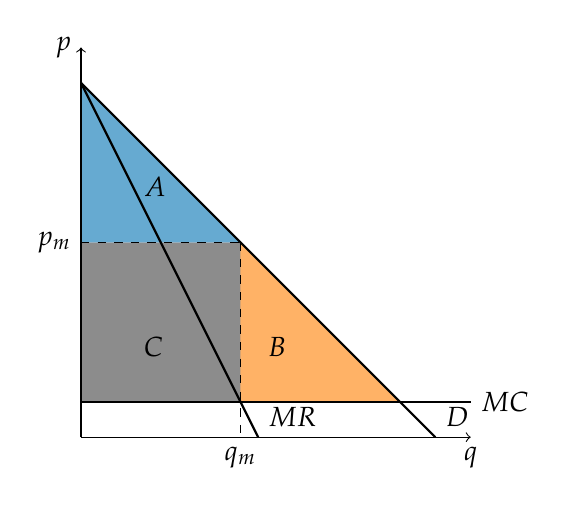
\begin{tikzpicture}[scale=0.45]
					\fill [darkgray!60] (0,1) -- (0,5.5) -- (4.5,5.5) -- (5.5,1) -- cycle;
					\fill [blue!60] (0,5.5) -- (4.5,5.5) -- (0,10) -- cycle;
					\fill [orange!60] (4.5,1) -- (4.5,5.5) -- (9,1) -- cycle;

					\draw [->] (0,0) to (0,11) node [left] {$p$};
					\draw [->] (0,0) to (11,0) node [below] {$q$};
					\draw [thick] (0,10)  to  (10,0)  node [above right] {$D$};
					\draw [thick] (0,10) to (5,0) node [above right] {$MR$};
					\draw [thick] (0,1)  to  (11,1)  node [right] {$MC$};

					\draw [dashed] (0,5.5) node [left] {$p_m$} to (4.55,5.5);
					\draw [dashed] (4.5,5.5) to (4.5,0) node [below] {$q_m$};

					\node [above right] at (1.5,6.5) {$A$};
					\node [above right] at (5,2) {$B$};
					\node [above right] at (1.5,2) {$C$};
				\end{tikzpicture}
			\end{figure}
		\end{column}
		\begin{column}{0.5\textwidth}
			\begin{wideitemize}
				\item \textbf{Area A:} Consumers WTP $> p_m$
				\begin{wideitemize}
					\item Could charge them more!
				\end{wideitemize}
				\item \textbf{Area B:} Consumers WTP between $MC$ and $p_m$
				\begin{wideitemize}
					\item Could sell to them at lower price
				\end{wideitemize}
				\item \textbf{Area C:} Current profit
			\end{wideitemize}
		\end{column}
	\end{columns}
\end{frame}

\begin{frame}{Types of price discrimination (Cabral terminology)}
	\begin{wideenumerate}
		\item \textbf{Perfect price discrimination}
		\begin{wideitemize}
			\vspace{3pt}
			\item Charge each consumer their exact WTP
			\item Extracts all surplus; unrealistic benchmark
		\end{wideitemize}
		\item \textbf{Selection by indicators}
		\begin{wideitemize}
			\vspace{3pt}
			\item Divide buyers into groups by observable characteristics
			\item Set different price for each group
		\end{wideitemize}
		\item \textbf{Self-selection}
		\begin{wideitemize}
			\vspace{3pt}
			\item Cannot observe type directly
			\item Design menu to induce consumers to reveal type
			\item (Covered next lecture)
		\end{wideitemize}
	\end{wideenumerate}
\end{frame}

\begin{frame}{Plan for today}
  \begin{wideenumerate}
    \item Consumer surplus: the log-sum formula
    \item The IIA problem: Red Bus / Blue Bus
    \item From demand to supply
    \item Types of price discrimination
    \item \textbf{Selection by indicators}
    \item Worked example: optimal pricing across markets
  \end{wideenumerate}
\end{frame}

\begin{frame}{Selection by indicators}
	\begin{wideitemize}
		\item Divide buyers into groups based on \textbf{observable characteristics}
		\item Set different price for each group
		\item Examples:
		\begin{wideitemize}
			\vspace{5pt}
			\item Student discounts (show student ID)
			\item Senior discounts
			\item Geographic pricing (different prices in different countries)
			\item Time-based pricing (matinees vs evening shows)
		\end{wideitemize}
	\end{wideitemize}
\end{frame}

\begin{frame}{Real-world examples of selection by indicators}
	\begin{wideenumerate}
		\item \textbf{Geographic:}
		\begin{wideitemize}
			\vspace{3pt}
			\item New car prices differ by region (Arizona vs California)
			\item Software priced differently in US vs India
		\end{wideitemize}
		\item \textbf{Age-based:}
		\begin{wideitemize}
			\vspace{3pt}
			\item Senior discounts (more elastic, retired, fixed income)
			\item Student discounts (more elastic, lower income)
		\end{wideitemize}
		\item \textbf{Time-based:}
		\begin{wideitemize}
			\vspace{3pt}
			\item Happy hour (flexible drinkers are more elastic)
			\item Black Friday (patient shoppers are more elastic)
		\end{wideitemize}
	\end{wideenumerate}
\end{frame}

\begin{frame}{Selection by indicators: setup}
	\begin{wideitemize}
		\item Two markets: market 1 and market 2
		\item Demand: $q_1 = D_1(p_1)$ and $q_2 = D_2(p_2)$
		\item Cost: $C(q_1 + q_2)$, with constant $MC$
		\item \textbf{Goal:} Find optimal price in each market
	\end{wideitemize}
\end{frame}

\begin{frame}{Selection by indicators: solution}
	\begin{wideitemize}
		\item Apply optimal pricing rule in each market:
		\begin{align*}
			MR_1 = MC \quad \text{and} \quad MR_2 = MC
		\end{align*}
		\item Equivalently, using elasticity rule:
		\begin{align*}
			\frac{p_1 - MC}{p_1} = \frac{1}{|\varepsilon_1|} \quad \text{and} \quad \frac{p_2 - MC}{p_2} = \frac{1}{|\varepsilon_2|}
		\end{align*}
		\item \textbf{Key implication:} Charge higher price in market with more inelastic demand
	\end{wideitemize}
\end{frame}

\begin{frame}{Plan for today}
  \begin{wideenumerate}
    \item Consumer surplus: the log-sum formula
    \item The IIA problem: Red Bus / Blue Bus
    \item From demand to supply
    \item Types of price discrimination
    \item Selection by indicators
    \item \textbf{Worked example: optimal pricing across markets}
  \end{wideenumerate}
\end{frame}

\begin{frame}{Worked example: Optimal pricing across markets}
	\begin{wideitemize}
		\item \textbf{Question:}
		\item Two markets with $\varepsilon_1 = -2$ and $\varepsilon_2 = -4$
		\item $MC = 6$
		\item Find optimal prices in each market.
	\end{wideitemize}
	\vspace{15pt}
	\centering
	\textit{Take 3 minutes to solve this.}
\end{frame}

\begin{frame}{Worked example: Optimal pricing (solution)}
	\begin{solutionbox}[Solution]
		\begin{itemize}
			\item Using Lerner index: $\frac{p - MC}{p} = \frac{1}{|\varepsilon|}$
			\item \textbf{Market 1} ($\varepsilon_1 = -2$):
			\begin{align*}
				\frac{p_1 - 6}{p_1} = \frac{1}{2} \quad \Rightarrow \quad p_1 - 6 = 0.5 p_1 \quad \Rightarrow \quad p_1 = 12
			\end{align*}
			\item \textbf{Market 2} ($\varepsilon_2 = -4$):
			\begin{align*}
				\frac{p_2 - 6}{p_2} = \frac{1}{4} \quad \Rightarrow \quad p_2 - 6 = 0.25 p_2 \quad \Rightarrow \quad p_2 = 8
			\end{align*}
			\item Price is higher in more inelastic market (market 1)
		\end{itemize}
	\end{solutionbox}
\end{frame}

\begin{frame}{Worked example: Student discount pricing}
	\begin{wideitemize}
		\item \textbf{Question:}
		\item A software company can distinguish students from professionals.
		\item Students: $\varepsilon_s = -3$; Professionals: $\varepsilon_p = -1.5$
		\item $MC = \$20$
		\item Calculate optimal prices for each group.
	\end{wideitemize}
	\vspace{15pt}
	\centering
	\textit{Take 3 minutes to solve this.}
\end{frame}

\begin{frame}{Worked example: Student discount pricing (solution)}
	\begin{solutionbox}[Solution]
		\begin{itemize}
			\item Using Lerner index: $p = \frac{MC}{1 + 1/\varepsilon}$
			\item \textbf{Students} ($\varepsilon_s = -3$):
			\begin{align*}
				p_s = \frac{20}{1 + 1/(-3)} = \frac{20}{1 - 0.33} = \frac{20}{0.67} = \$30
			\end{align*}
			\item \textbf{Professionals} ($\varepsilon_p = -1.5$):
			\begin{align*}
				p_p = \frac{20}{1 + 1/(-1.5)} = \frac{20}{1 - 0.67} = \frac{20}{0.33} = \$60
			\end{align*}
			\item Students pay \$30 (50\% discount); professionals pay \$60
			\item Students more elastic $\rightarrow$ lower price
		\end{itemize}
	\end{solutionbox}
\end{frame}

\begin{frame}{Welfare effects of selection by indicators}
	\begin{wideitemize}
		\item \textbf{Producer surplus:} Increases (that's why firms do it)
		\item \textbf{Consumer surplus:} Ambiguous
		\begin{wideitemize}
			\vspace{5pt}
			\item Some consumers pay more (inelastic market)
			\item Some consumers pay less (elastic market)
			\item Some consumers now served who weren't before
		\end{wideitemize}
		\item \textbf{Total welfare:} Depends on whether new markets are served
		\begin{wideitemize}
			\vspace{5pt}
			\item If discrimination opens new markets $\rightarrow$ welfare may increase
			\item If just redistributes $\rightarrow$ welfare may decrease
		\end{wideitemize}
	\end{wideitemize}
\end{frame}

\begin{frame}{When is price discrimination welfare-improving?}
	\begin{wideitemize}
		\item \textbf{Welfare improves when:}
		\begin{wideitemize}
			\vspace{5pt}
			\item Discrimination opens up new markets (serves consumers who otherwise wouldn't be served)
			\item Example: Student discounts let students afford textbooks
		\end{wideitemize}
		\item \textbf{Welfare may decrease when:}
		\begin{wideitemize}
			\vspace{5pt}
			\item Just redistributes from consumers to firm
			\item No expansion of output
		\end{wideitemize}
		\item \textbf{Key insight:} Output matters!
		\begin{wideitemize}
			\vspace{5pt}
			\item If total quantity sold goes up, welfare likely increases
			\item If total quantity stays same, welfare likely decreases
		\end{wideitemize}
	\end{wideitemize}
\end{frame}

\begin{frame}{Connection: Demand estimation and price discrimination}
	\begin{wideitemize}
		\item \textbf{Demand estimation gives us:}
		\begin{wideitemize}
			\vspace{5pt}
			\item Elasticities by consumer group (if demographics used)
			\item Which groups are more/less price-sensitive
		\end{wideitemize}
		\item \textbf{This informs pricing strategy:}
		\begin{wideitemize}
			\vspace{5pt}
			\item High elasticity groups $\rightarrow$ lower price
			\item Low elasticity groups $\rightarrow$ higher price
		\end{wideitemize}
		\item \textbf{Example:} Nevo (2001) found that families with children are less price-sensitive for kid cereals
		\item Cereal companies can use this for targeted promotions
	\end{wideitemize}
\end{frame}

%%%%%%%%%%%%%%%%%%%%%%%%%%%%%%%%%%%%%%%%%%%%%%%%%%%%%%%%%%%%%
% KEY POINTS
%%%%%%%%%%%%%%%%%%%%%%%%%%%%%%%%%%%%%%%%%%%%%%%%%%%%%%%%%%%%%

\begin{frame}{Key Points}
	\vspace{11pt}
	\begin{wideenumerate}
		\item \textbf{Log-sum formula}: $CS_i = \frac{1}{\alpha}\ln\left[\sum_j \exp(\delta_j)\right]$
		\item \textbf{Red Bus / Blue Bus}: Logit overcounts value of similar products
		\item \textbf{IIA}: Substitution proportional to share, not similarity
		\item Demographics partially help; mixed logit fully relaxes IIA
		\item \textbf{Price discrimination}: Different prices for same good
		\item \textbf{Perfect PD}: Charge each consumer their WTP (benchmark)
		\item \textbf{Selection by indicators}: Group pricing based on observables
		\item Charge higher price in \textbf{more inelastic} market: $p = MC / (1 + 1/\varepsilon)$
	\end{wideenumerate}
\end{frame}

\begin{frame}{Next time}
	\begin{wideitemize}
		\item \textbf{Lecture 5:} Two-Part Tariffs and Self-Selection
		\begin{wideitemize}
			\vspace{5pt}
			\item Two-part tariffs: $F + p \times q$
			\item Self-selection: menu design, versioning
			\item Incentive compatibility constraints
		\end{wideitemize}
	\end{wideitemize}
\end{frame}

\end{document}
